\chapter[Справочная информация]{Справочная информация}
\label{chap:reference_information}

\section[Технические харакетристики]{Технические характеристики гравиметра \cg{}}

Технические характеристики планшетного компьютера и прибора \cg{} могут быть
изменены без уведомления.

\begin{longtable}{|p{0.35\textwidth}|p{0.58\textwidth}|}
  \hline
  Тип датчика & Плавленый кварц, с использованием электростатического
  обнуления \\
  \hline
  Точность показания & 0,1 микроГал \\
  \hline
  Стандартное отклонение & <5 микроГал \\
  \hline
  Рабочий диапазон & В любой точке мира (8 000 мГал без переустановки) \\
  \hline
  Остаточный дрейф & < 20 мкГал/день \\
  \hline
  Некомпенсированный дрейф & < 200 мкГал/день \\
  \hline
  Диапазон автоматической компенсации наклона & \textpm{}200 угловых секунд \\
  \hline
  Устойчивость к удару & Обычно < 5 мкГал для толчков до 20 g \\
  \hline
  Автоматически вводимые поправки & На земные приливы, на наклон прибора, на
  температуру, на дрейф \\
  \hline
  Скорость вывода данных & До 10 Гц, выбирается пользователем \\
  \hline
  Точность GPS & Стандартная точность 2,5 м \\ 
  \hline
  Работа без нажатия клавиш & Планшетный компьютер с функцией Bluetooth \\
  \hline
  Ёмкость аккумуляторной батареи & Перезаряжаемые литиевые аккумуляторные
  батареи со встроенной логикой: 2\texttimes{}6,8 A-ч (10,8~В). Работа в
  течение суток при температуре 25\textcelsius{} (77\textdegree{}F) \\
  \hline
  Потребляемая мощность & 5,2~Вт при температуре 25\textcelsius{}
  (77\textdegree{}C) \\
  \hline
  Рабочая температура & от \textminus{}40\textcelsius{} до +45\textcelsius{}
  (от \textminus{}40\textdegree{}F до 113\textcelsius{}) Опционная
  высокотемпературная версия с диапазоном до +55\textcelsius{}
  (131\textdegree{}F) \\
  \hline
  Вывод цифровых данных & USB и Bluetooth \\
  \hline
  Размеры & 21,5 см (В) \texttimes{} 21 см \texttimes{} 24 см (8,5 дюйма
  \texttimes{} 8,2 дюйма \texttimes{} 9 дюймов) \\
  \hline
  Вес & 5,2 кг (11,5 фунтов) с аккумуляторными батареями \\
  \hline
  Стандартная комплектация системы &  Гравиметр \cg{} \newline Штатив CG-6
  \newline 2 перезаряжаемые аккумуляторные батареи со встроенным процессором
  \newline Зарядное устройство \newline Блок питания и кабель USB \newline
  Контейнер для перевозки \newline Плечевой ремень \newline Руководство
  пользователя \newline Указания по быстрому вводу в действие \newline Сумка
  для переноски \newline Комплект переходников для штепсельной розетки
  \newline Комплект запасных частей \\
  \hline
  Отгрузочный вес и размеры & 97 см \texttimes{} 60 \texttimes{} 55 (В) (38
  дюймов \texttimes{} 24 дюйма \texttimes{} 22 дюйма (В)), 26 кг, (60 фунтов). \\
  \hline
  Доступные опции и принадлежности & Высокотемпературная (HT) версия прибора
  \newline Планшетный компьютер + аксессуары \newline  Программное обеспечение
  LynxLG \newline  Кабель внешнего источника питания 12 В \newline  Комплект
  для холодной погоды \newline  Рюкзак Seco \newline Запасные аккумуляторные
  батареи \newline  Запасные источники питания для планшетного компьютера
  \newline  Trident~-- штатив для измерения градиента \newline  Запасной
  контейнер для аккумуляторных батарей \newline  Штатив с удлинёнными опорами
  \\
  \hline
\end{longtable}

\section[Расположение датчика]{Расположение датчика гравиметра \cg{}}

На рисунке показано местоположение датчика прибора \cg{}.

\newpage
\begin{figure}[h]
  \centering
  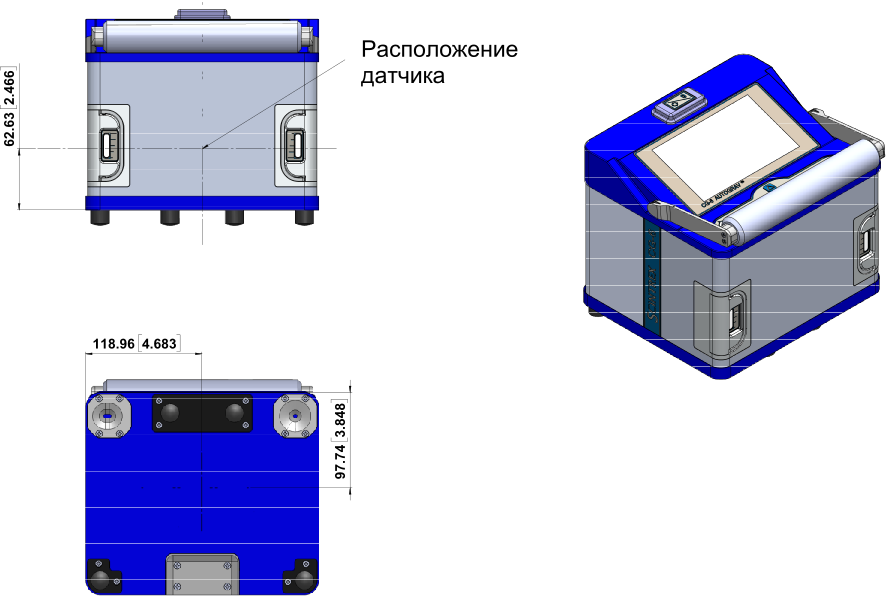
\includegraphics[width=\textwidth]{figures/the_cg6_autograv_sensor_location}
  \caption{Местоположение датчика прибора \cg{}}
  \label{fig:the_cg6_autograv_sensor_location}
\end{figure}

\section{Спецификация прибора}

Стандартные принадлежности прибора \cg{}

\begin{longtable}{|p{0.75\textwidth}|p{0.15\textwidth}|}
  \hline
  Наименование компонента & Номер \\
  \hline
  Система \cg{} включает в себя: & 101370002 \\
  \hline
  Прибор \cg{} & 129370505 \\
  \hline
  Штатив прибора & 126370138 \\
  \hline
  Батарейный блок (x2) & 0221029M \\
  \hline
  Контейнер аккумуляторной батареи (x2) & 126370501 \\
  \hline
  Блок питания переменного \ постоянного тока & 128370055 \\
  \hline
  Зарядное устройство с микропроцессорным управлением & 400209 \\
  \hline
  Внешний USB-кабель & 128370053 \\
  \hline
  Комплект запасных частей & 888025 \\
  \hline
  Комплект переходников для штепсельной розетки & 400128 \\
  \hline
  Указания по быстрому вводу прибора CG-6 в действие & 115370002 \\
  \hline
  Флэш-накопитель с руководствами к CG-6 & 888407 \\
  \hline
  Сумка для переноски CG-6 & 888012 \\
  \hline
  Сборка транспортировочного ящика CG-6 & 888016 \\
  \hline
\end{longtable}

Опционные принадлежности прибора \cg{}

\begin{longtable}{|p{0.75\textwidth}|p{0.15\textwidth}|}
  \hline
  Наименование компонента & Номер \\
  \hline
  Планшетный компьютер & 888030 \\
  \hline
  Источник питания, обеспечивающий работу планшетного компьютера 
  в течение 10 часов & 400020 \\
  \hline
  Интеллектуальная аккумуляторная батарея & 0221029M \\
  \hline
  Рюкзак Seco & 140220 \\
  \hline
  Узел держателя батареи & 126370501 \\
  \hline
  Комплект для холодной погоды & 888405 \\
  \hline
  Кабель внешнего источника питания 12 В & 128370060 \\
  \hline
  Штатив с удлиненными ножками & 867209 \\
  \hline
  Штатив для измерения градиента Trident и контейнер для перевозки & 101370004 \\
  \hline
\end{longtable}

\section{Установка аккумуляторных батарей}

Согласно строгим правилам Международной ассоциации воздушного транспорта (IATA),
перевозка аккумуляторных батарей гравиметра \cg{} разрешается только в отдельной
упаковке. Уровень заряда аккумуляторных батарей не должен превышать 30\%.
Прежде, чем вы сможете, подать питание на свой прибор \cg{}, потребуются некоторые
усилия, чтобы собрать батарейный контейнер (p/n 126370001) с интеллектуальными
аккумуляторными батареями (p/n 0221029M). Процесс сборки изображён на рисунке:

\infobox{
  Если вы приобретаете аккумуляторные батареи для прибора CG-6 не в компании
  Scintrex, вам нужно срезать язычок, как показано ниже, и закрыть это место
  куском упаковочной плёнки 3M 3850 или аналогичной тонкой плёнкой.
}

\begin{figure}[h]
  \centering
  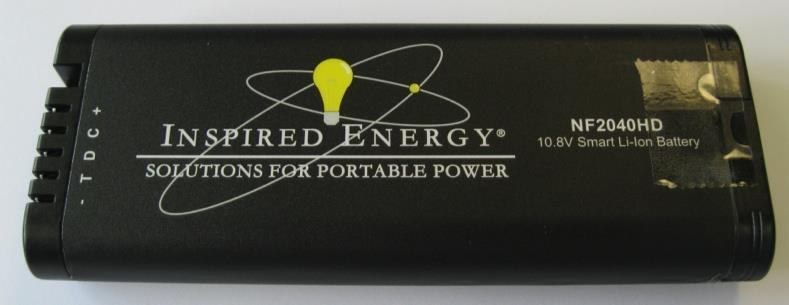
\includegraphics[width=0.7\textwidth]{figures/removing_the_pull_tab_and_covering_with_tape}
  \caption{Срезанный язычок, закрытый плёнкой}
  \label{fig:removing_the_pull_tab_and_covering_with_tape}
\end{figure}

\infobox{
  Показанная на четвёртом кадре отвёртка с шестигранником поставляется с
  комплектом запасных частей прибора CG-6 (\textnumero{} 888025).
}

\begin{figure}[h]
  \centering
  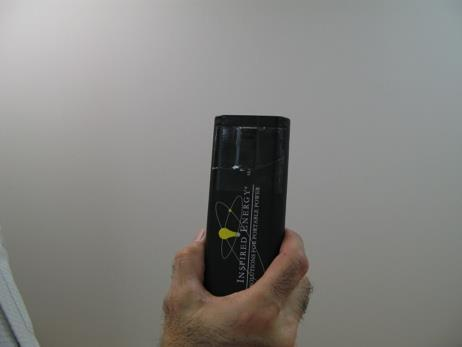
\includegraphics[width=0.4\textwidth]{figures/assembling_the_battery_packs_1}
  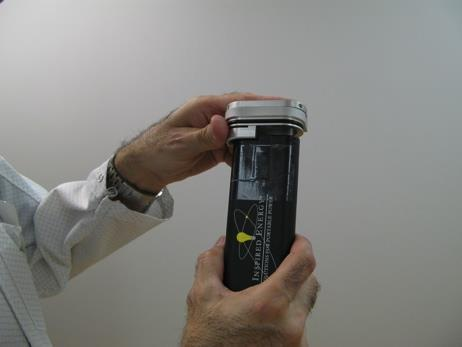
\includegraphics[width=0.4\textwidth]{figures/assembling_the_battery_packs_2}
  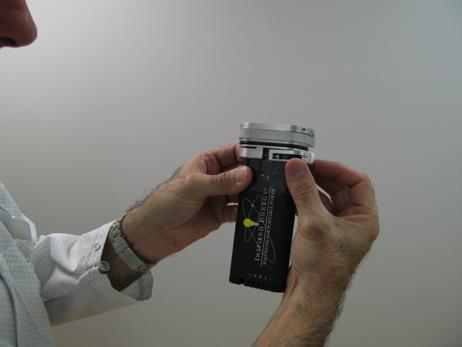
\includegraphics[width=0.4\textwidth]{figures/assembling_the_battery_packs_3}
  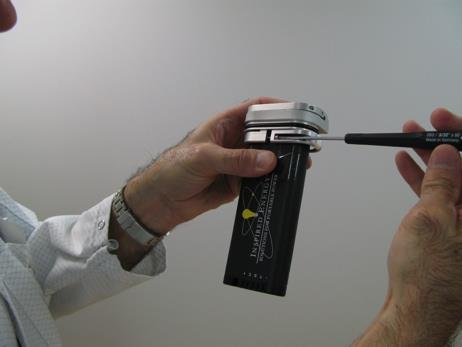
\includegraphics[width=0.4\textwidth]{figures/assembling_the_battery_packs_4}
  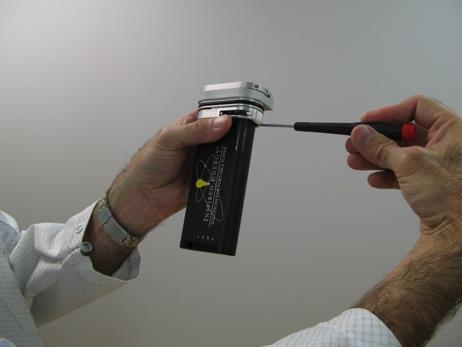
\includegraphics[width=0.4\textwidth]{figures/assembling_the_battery_packs_5}
  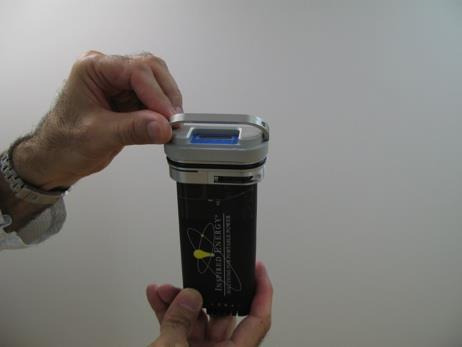
\includegraphics[width=0.4\textwidth]{figures/assembling_the_battery_packs_6}
  \caption{Сборка батарейного блока}
  \label{fig:assembling_the_battery_packs}
\end{figure}

\warningbox{
  Ручка на крышке собранного батарейного блока должна находиться с той стороны
  аккумуляторной батареи, где нанесён её логотип~-- см. последний кадр на
  рисунке.
}

\section{Гарантия}
\label{sec:warranty}

На все оборудование, производимое компанией Scintrex, за исключением расходных
деталей и материалов, даётся гарантия отсутствия дефектов материалов и
изготовления в течение одного года от даты отгрузки. В случае, если при
нормальной эксплуатации в течение гарантийного периода проявятся те или иные
дефекты, компания Scintrex сделает необходимый ремонт бесплатно.

Данная гарантия не распространяется на повреждения, ставшие следствием
неправильного использования или несчастного случая. Гарантия может быть
аннулирована, если панель прибора открывалась лицами, не уполномоченными
компанией Scintrex.

\section{Ремонт}
\label{sec:repair}

\subsection{Решение по отправке прибора в ремонт}

Прежде чем отправить прибор для ремонта, сообщите о характере возникшей проблемы
специалистам нашего Отдела обслуживания клиентов по электронной почте, телефону,
факсу или электронной почте. Наш Отдел обслуживания клиентов может предложить
вам провести несложные проверки, которые могут решить вашу проблему без затрат
времени и средств на перевозку прибора в производственное подразделение компании
Scintrex для ремонта. Если проблема не может быть решена, наш персонал попросить
вас отправить прибор на наш завод для необходимого ремонта.

\subsection{Описание проблемы}

Описывая проблему, не забудьте указать следующую информацию:
\begin{itemize}
  \item Симптомы проблемы.

  \item Как началась проблема.

  \item Является ли неполадка постоянной, нерегулярной или повторяющейся.

  \item Если неполадка постоянная, при каких обстоятельствах она возникает.

  \item Есть ли компьютерные данные, демонстрирующие проблему.
\end{itemize}

\section{Инструкция по доставке}
\label{sec:shipping_instructions}

Инструмент не принимается для ремонта без предварительной оплаты перевозки.
После ремонта прибор возвращается с наложенным платежом, при отсутствии других
договорённостей с компанией Scintrex. Просьба указывать серийный номер прибора
во всех сообщениях, касающихся арендованного или приобретённого у компании
Scintrex оборудования.

Прибор нужно отправить по адресу:\\
SCINTREX Limited\\
222 Snidercroft Road, Concord, ON, Canada, L4K 2K1

Telephone:\\
+1 905 669 2280\\
Fax:\\
+1 905 669 9899
